\chapter{Singular Value Decomposition}
\label{chap:SingularValueDecomposition}

We will picture the action of a linear map,
specifically, the action of a linear transformation $\map{h}{\Re^2}{\Re^2}$.
That will connect with an important way to factor matrices
and an interesting application.


\section{Drawing the action}
A defining property of linear maps is that 
$h(r\cdot\vec{v})=r\cdot h(\vec{v})$.
Recall that a line through the origin in $\Re^n$ has the form 
$\set{r\cdot \vec{v}\suchthat r\in\Re}$ for some~$\vec{v}$. 
Thus the scalar multiplication property  
imposes a uniformity condition on a linear map:~its action on any 
line through the origin is determined by its action
on any nonzero vector in that line.

For instance, consider the line~$y=2x$ in the plane
\begin{equation*}
  \set{r\cdot\colvec{1 \\ 2}\suchthat r\in\Re}
\end{equation*}
and suppose that $\map{t}{\Re^2}{\Re^2}$ is represented by this matrix.
\begin{equation*}
  \rep{t}{\stdbasis_2,\stdbasis_2}
  =
  \begin{mat}
    1 &2 \\
    3 &4
  \end{mat}
\end{equation*}
Then the map $t$ has this effect on one of the line's vectors.
\begin{equation*}
  \vec{v}=\colvec{1 \\ 2}\mapsunder{t}\colvec{5 \\ 11}
\end{equation*}
On $2\vec{v}$ the 
map has twice the effect, on  $3\vec{v}$ it has three times the
effect, etc.
\begin{equation*}
  \colvec{2 \\ 4}\mapsunder{t}\colvec{10 \\ 22}
  \qquad
  \colvec{3 \\ 6}\mapsunder{t}\colvec{15 \\ 33}
  \qquad
  \colvec{r \\ 2r}\mapsunder{t}\colvec{5r \\ 11r}
\end{equation*}
We will use this observation to illustrate the action of 
linear transformations of the plane, $\map{t}{\Re^2}{\Re^2}$
(we look at the plane just because the pictures are 
easy to draw). 

The $t(r\cdot\vec{v})=r\cdot t(\vec{v})$ relationship says that
a linear map has the same effect on all vectors in a line through the
origin.
So to show a transformation's action we can fix 
one nonzero vector element from each line through the origin
and then show where the transformation takes each of 
those vectors.
The natural set containing one point from each plane line through the origin 
is the upper half of the unit circle, shown here
(the colors are explained below).
% \begin{sagecommandline}
% sage: load("plot_action.sage")
% sage: p = plot_circle_action(1,0,0,1) 
% sage: p.set_axes_range(-1.5, 1.5, -0.5, 1.5) 
% sage: p.save("graphics/svd000.pdf")
% \end{sagecommandline}
\begin{sagesilent}
load("plot_action.sage")
p = plot_circle_action(1,0,0,1) 
p.set_axes_range(-1.5, 1.5, -0.5, 1.5) 
p.save("graphics/svd000.pdf")
\end{sagesilent}
\begin{equation*}
  U=\set{\colvec{\cos(t) \\ \sin(t)}
         \suchthat 
         0\leq t<\pi}
  \qquad
  \vcenteredhbox{\includegraphics{graphics/svd000.pdf}}  
\end{equation*}
The point $(1,0)$ is included in that set but
$(-1,0)$ is not, which is why there is an open circle.

The first illustration is for a simple transformation.
\begin{equation*}
  \colvec{x \\ y} \mapsto \colvec{2x \\ y}
\end{equation*}
\Sage{} can compute the effect of this transformation
on the upper half circle. 
The code below inputs the file \inlinecode{plot_action.sage}
to get access to the routine
\inlinecode{plot_circle_action(a,b,c,d)}. 
This finds the output curve by multipling points on 
the input upper half unit circle by this matrix
\begin{equation*}
  \begin{mat}
    a &b \\
    c &d
  \end{mat}
\end{equation*}
and then connecting those output dots to get the output curve.
The source code of \inlinecode{plot_action.sage} is 
at the end of this chapter.
\begin{sagecommandline}
sage: load("plot_action.sage")
sage: q = plot_circle_action(1,0,0,1) 
sage: q.set_axes_range(-2, 2, -1, 2) 
sage: q.save("graphics/svd001a.pdf")
sage: p = plot_circle_action(2,0,0,1) 
sage: p.set_axes_range(-2, 2, -1, 2) 
sage: p.save("graphics/svd001b.pdf")
\end{sagecommandline}
% \begin{sagesilent}
% load("plot_action.sage")
% q = plot_circle_action(1,0,0,1) 
% q.set_axes_range(-2, 2, -1, 2) 
% q.save("graphics/svd001a.pdf")
% p = plot_circle_action(2,0,0,1) 
% p.set_axes_range(-2, 2, -1, 2) 
% p.save("graphics/svd001b.pdf")
% \end{sagesilent}
Here is the before and after, the upper half circle 
and the associated output.
The colors show the association\Dash which 
points on the left are mapped to which points 
on the right.
\begin{equation*}
  \vcenteredhbox{\includegraphics{graphics/svd001a.pdf}}
  \quad\mapsunder{\big (\begin{smallmatrix} 2 &0 \\ 0 &1 \end{smallmatrix}\big )}\quad
  \vcenteredhbox{\includegraphics{graphics/svd001b.pdf}}
\end{equation*}
\Sage{} drew the unit circle by plotting the action of the identity map.
Then \Sage{} drew the effect of the transformation by plotting the
action of this matrix.
\begin{equation*}
\begin{mat}
  2  &0  \\
  0  &1
\end{mat}
\end{equation*}

The next before and after picture shows
the effect of the map
\begin{equation*}
  \colvec{x \\ y} \mapsto \colvec{-x \\ 3y}
\end{equation*}
that triples the $y$~component and also multiplies the 
$x$~component by $-1$.\footnote{%
  As in other chapters, some of the graphics here are drawn with  
  some options that are not shown.
  In this case, the \protect\inlinecode{p.save(...)} has
  the \protect{ticks\_integer=True} option.
  This just reduces clutter that isn't linear algebra.}
\begin{sagecommandline}
sage: q = plot_circle_action(1,0,0,1) 
sage: q.set_axes_range(-2, 2, -1.25, 3.25) 
sage: q.save("graphics/svd002a.pdf")
sage: p = plot_circle_action(-1,0,0,3) 
sage: p.set_axes_range(-2, 2, -1.25, 3.25) 
sage: p.save("graphics/svd002b.pdf")
\end{sagecommandline}
\begin{sagesilent}
load("plot_action.sage")
q = plot_circle_action(1,0,0,1) 
q.set_axes_range(-2, 2, -1.25, 3.25) 
q.save("graphics/svd002a.pdf", ticks_integer=True)
p = plot_circle_action(-1,0,0,3) 
p.set_axes_range(-2, 2, -1.25, 3.25) 
p.save("graphics/svd002b.pdf", ticks_integer=True)
\end{sagesilent}
\begin{equation*}
  \vcenteredhbox{\includegraphics{graphics/svd002a.pdf}}
  \quad\mapsunder{\big (\begin{smallmatrix} -1 &0 \\ 0 &3 \end{smallmatrix}\big )}\quad
  \vcenteredhbox{\includegraphics{graphics/svd002b.pdf}}
\end{equation*}
This is where the colors have something to say.
On the input circle, when you move counterclockwise, the colors go from 
red to orange, then to green, blue, indigo, and 
finally violet.
But the output does the opposite: to move from red to violet, you
move clockwise.
This transformation changes the orientation,
or sense, of the curve. 

The next transformation is a shear.\footnote{%
  A dictionary definition of a shear is that it is when 
  two parts of a body  
  slide relatively to each other, in a direction parallel to their 
  plane of contact.  
  Thus, when you write on a paper the flakes of pencil 
  graphite shear off the pencil.}
\begin{equation*}
  \colvec{x \\ y} \mapsto \colvec{x+2y \\ y}
\end{equation*}
The output's first component is affected
by the input vector's distance from the $y$-axis.
\begin{sagecommandline}
sage: q = plot_circle_action(1,0,0,1) 
sage: q.set_axes_range(-1.5, 1.5, -2.25, 2.25) 
sage: q.save("graphics/svd003a.pdf")
sage: p = plot_circle_action(1,0,2,1) 
sage: p.set_axes_range(-1.5, 1.5, -2.25, 2.25) 
sage: p.save("graphics/svd003b.pdf")
\end{sagecommandline}
\begin{sagesilent}
load("plot_action.sage")
q = plot_circle_action(1,0,0,1) 
q.set_axes_range(-1.5, 1.5, -2.25, 2.25, ticks_integer=True) 
q.save("graphics/svd003a.pdf")
p = plot_circle_action(1,0,2,1) 
p.set_axes_range(-1.5, 1.5, -2.25, 2.25, ticks_integer=True) 
p.save("graphics/svd003b.pdf")
\end{sagesilent}
\begin{equation*}
  \vcenteredhbox{\includegraphics{graphics/svd003a.pdf}}
  \quad\mapsunder{\big (\begin{smallmatrix} 1 &0 \\ 2 &1 \end{smallmatrix}\big )}\quad
  \vcenteredhbox{\includegraphics{graphics/svd003b.pdf}}
\end{equation*}

Here is another shear.
In this case the output's 
second component is affected by the input's distance from 
the $x$-axis.
\begin{sagecommandline}
sage: q = plot_circle_action(1,0,0,1) 
sage: q.set_axes_range(-2, 2, -2, 2) 
sage: q.save("graphics/svd004a.pdf")
sage: p = plot_circle_action(1,1/2,0,1) 
sage: p.set_axes_range(-2, 2, -2, 2) 
sage: p.save("graphics/svd004b.pdf")
\end{sagecommandline}
% \begin{sagesilent}
% load("plot_action.sage")
% q = plot_circle_action(1,0,0,1) 
% q.set_axes_range(-2, 2, -2, 2) 
% q.save("graphics/svd004a.pdf")
% p = plot_circle_action(1,1/2,0,1) 
% p.set_axes_range(-2, 2, -2, 2) 
% p.save("graphics/svd004b.pdf")
% \end{sagesilent}
\begin{equation*}
  \vcenteredhbox{\includegraphics{graphics/svd004a.pdf}}
  \quad\mapsunder{\big (\begin{smallmatrix} 1 &1/2 \\ 0 &1 \end{smallmatrix}\big )}\quad
  \vcenteredhbox{\includegraphics{graphics/svd004b.pdf}}
\end{equation*}

And here is a generic transformation.
It changes orientation also.
\begin{sagecommandline}
sage: q = plot_circle_action(1,0,0,1) 
sage: q.set_axes_range(-2, 4, -3, 6) 
sage: q.save("graphics/svd005a.pdf")
sage: p = plot_circle_action(1,2,3,4) 
sage: p.set_axes_range(-2, 4, -3, 6) 
sage: p.save("graphics/svd005b.pdf")
\end{sagecommandline}
% \begin{sagesilent}
% load("plot_action.sage")
% q = plot_circle_action(1,0,0,1) 
% q.set_axes_range(-2, 4, -3, 6) 
% q.save("graphics/svd005a.pdf",figsize=3)
% p = plot_circle_action(1,2,3,4) 
% p.set_axes_range(-2, 4, -3, 6) 
% p.save("graphics/svd005b.pdf",figsize=3)
% \end{sagesilent}
\begin{equation*}
  \vcenteredhbox{\includegraphics{graphics/svd005a.pdf}}
  \quad\mapsunder{\big (\begin{smallmatrix} 1 &2 \\ 3 &4 \end{smallmatrix}\big )}\quad
  \vcenteredhbox{\includegraphics{graphics/svd005b.pdf}}
\end{equation*}



\section{SVD}
The above pictures show the unit circle mapping to ellipses.
Recall that in $\Re^2$ an ellipse has a \textit{major axis}, 
the longer one, and a 
\textit{minor axis}.\footnote{If the two axes have the same length 
then the ellipse is a circle.
If one axis has length zero then the ellipse is a line segment 
and if both have length zero then it is a point.}
Write $\sigma_1$ for the length of the semi-major axis, 
the distance from the center to the furthest-away point on the ellipse,
and write $\sigma_2$ for the length of the semi-minor axis.
\begin{sagecommandline}
sage: plot.options['axes_pad'] = 0.5
sage: plot.options['fontsize'] = 4
sage: plot.options['aspect_ratio'] = 1
sage: sigma_1=3
sage: sigma_2=1
sage: E = ellipse((0,0), sigma_1, sigma_2)
sage: E.save("graphics/svd100.pdf",figsize=3)
\end{sagecommandline}
\begin{sagesilent}
plot.options['axes_pad'] = 0.5
plot.options['fontsize'] = 2
plot.options['aspect_ratio'] = 1
plot.options['figsize'] = 1
sigma_1=3
sigma_2=1
E = ellipse((0,0), sigma_1, sigma_2)
# E.save("graphics/svd100.pdf", axes_pad=0.075, dpi=1200, fontsize=7, ticks=([-3,-2,-1,1,2,3],[-1,1]), figsize=1.5)
E.save("graphics/svd100.pdf", axes_pad=0.075, figsize=3)
\end{sagesilent}
\begin{center}
  \includegraphics{graphics/svd100.pdf}
\end{center}
In an ellipse the two axes are orthogonal.
In the above graph the major axis lies along the $x$-axis while the
minor axis lies along the $y$-axis.

Under any linear map $\map{t}{\Re^n}{\Re^m}$ the 
unit sphere maps to a hyperellipse.
This is a version of the \textit{Singular Value Decomposition} of
matrices:
for any linear map $\map{t}{\Re^m}{\Re^n}$ there are bases
$B=\sequence{\vec{\beta}_1,\ldots,\vec{\beta}_m}$ for the domain and
$D=\sequence{\vec{\delta}_1,\ldots,\vec{\delta}_n}$ for the codomain
such that $t(\vec{\beta}_i)=\sigma_i\vec{\delta}_i$, where the
\textit{singular values}
$\sigma_i$ are scalars.
The next section sketches a proof
but we first illustrate this result by using an example matrix.
\Sage{} will find the two bases $B$ and~$D$ and will picture how the 
vectors $\vec{\beta}_i$ 
are mapped to the $\sigma_i\vec{\delta}_i$.

So consider again the generic matrix.
Here is its action again, this time shown
on a full circle.
\begin{sagecommandline}
sage: load("plot_action.sage")
sage: q = plot_circle_action(1,0,0,1,full_circle=True) 
sage: q.set_axes_range(-2, 2, -5, 6) 
sage: q.save("graphics/svd101a.pdf")
sage: p = plot_circle_action(1,2,3,4,full_circle=True) 
sage: p.set_axes_range(-4, 4, -5, 6) 
sage: p.save("graphics/svd101b.pdf")
\end{sagecommandline}
% \begin{sagesilent}
% load("plot_action.sage")
% q = plot_circle_action(1,0,0,1,full_circle=True) 
% q.set_axes_range(-2, 2, -5, 6) 
% q.save("graphics/svd101a.pdf")
% p = plot_circle_action(1,2,3,4,full_circle=True) 
% p.set_axes_range(-4, 4, -5, 6) 
% p.save("graphics/svd101b.pdf")
% \end{sagesilent}
\begin{equation*}
  \vcenteredhbox{\includegraphics{graphics/svd101a.pdf}}
  \quad\mapsunder{\big (\begin{smallmatrix} 1 &2 \\ 3 &4 \end{smallmatrix}\big )}\quad
  \vcenteredhbox{\includegraphics{graphics/svd101b.pdf}}
  \tag{$*$}
\end{equation*}
\Sage{} will find the SVD of this example matrix.
\begin{sagecommandline}
sage: M = matrix(RDF, [[1, 2], [3, 4]])
sage: U,Sigma,V = M.SVD()
sage: U
sage: Sigma
sage: V
sage: U*Sigma*(V.transpose())
\end{sagecommandline}
\noindent 
The Singular Value Decomposition has $M$ as the product of
three matrices, $U\Sigma\trans{V}$.
The basis vectors $\vec{\beta}_1$, $\vec{\beta}_2$, $\vec{\delta}_1$, 
and~$\vec{\delta}_2$ are the columns of $U$ and~$V$. 
The singular values are the diagonal entries of~$\Sigma$.
\Sage{} will plot the effect of the transformation
on the basis vectors for the domain so we can compare those with the
basis vectors for the codomain.
\begin{sagecommandline}
sage: M = matrix(RDF, [[1, 2], [3, 4]])
sage: U,Sigma,V = M.SVD()
sage: beta_1 = vector(RDF, [U[0][0], U[1][0]])
sage: beta_2 = vector(RDF, [U[0][1], U[1][1]])
sage: delta_1 = vector(RDF, [V[0][0], V[1][0]])
sage: delta_2 = vector(RDF, [V[0][1], V[1][1]])
sage: plot.options['axes_pad'] = 0.05
sage: plot.options['fontsize'] = 7
sage: plot.options['aspect_ratio'] = 1
sage: s = 2  # uniform arrowsize
sage: C = circle((0,0), 1)
sage: P = C + plot(beta_1,arrowsize=s) + plot(beta_2,arrowsize=s)
sage: P.save("graphics/svd102a.pdf",figsize=2)
sage: image_color=Color(1,0.5,0.5)   # color for t(beta_1), t(beta_2)
sage: Q = C + plot(beta_1*M, width=3,color=image_color,arrowsize=s) 
sage: Q = Q + plot(delta_1,width=1.4,color='blue',arrowsize=s) 
sage: Q = Q + plot(beta_2*M,width=3,color=image_color,arrowsize=s) 
sage: Q = Q + plot(delta_2,width=1.4,color='blue',arrowsize=s)
sage: Q.save("graphics/svd102b.pdf",figsize=4.467)
\end{sagecommandline}
% \begin{sagesilent}
% M = matrix(RDF, [[1, 2], [3, 4]])
% U,Sigma,V = M.SVD()
% beta_1 = vector(RDF, [U[0][0], U[1][0]])
% beta_2 = vector(RDF, [U[0][1], U[1][1]])
% delta_1 = vector(RDF, [V[0][0], V[1][0]])
% delta_2 = vector(RDF, [V[0][1], V[1][1]])
% plot.options['axes_pad'] = 0.05
% plot.options['fontsize'] = 7
% plot.options['aspect_ratio'] = 1
% arrowsize = 2
% C = circle((0,0), 1)
% P = C + plot(beta_1,arrowsize=arrowsize) + plot(beta_2,arrowsize=arrowsize)
% P.save("graphics/svd102a.pdf", figsize=1, axes_pad=0.05)
% image_color=Color(1,0.5,0.5)   # color for t(beta_1), t(beta_2)
% Q = C + plot(beta_1*M, width=3, arrowsize=arrowsize, color=image_color) 
% Q = Q + plot(delta_1,width=1.4, arrowsize=arrowsize,color='blue') 
% Q = Q + plot(beta_2*M,width=3, arrowsize=arrowsize,color=image_color) 
% Q = Q + plot(delta_2,width=1.4, arrowsize=arrowsize,color='blue')
% Q.save("graphics/svd102b.pdf", figsize=2.2335, axes_pad=0.05)
% \end{sagesilent}
% was: Q.save("graphics/svd102b.pdf", figsize=4.467, axes_pad=0.05)
In the picture below the domain's 
blue $\vec{\beta}$'s on the left map to the codomain's light red 
$t(\vec{\beta})$'s on the right.
Also on the right, in blue, are the $\vec{\delta}$'s.
The diagonal entries of $\Sigma$ tell us about the
red vectors:~$t(\vec{\beta}_1)$ is about $5.5$ times $\vec{\delta}_1$
while $t(\vec{\beta}_2)$ is about $0.4$ times~$\vec{\delta}_2$.
Thus, in the diagram~($*$) showing the action of this generic matrix,
that is the length of the semimajor and semiminor axes. 
\begin{equation*}
  % \setlength{\fboxsep}{0in} % used to set box heights by eye; surrounded each picture env with a fbox
  \setlength{\unitlength}{1in}
  \begin{picture}(1.35,1.35)
    \put(0,1.825){\includegraphics{graphics/svd102a.pdf}}
    \put(.3,1.9){\scriptsize $\vec{\beta}_1$}
    \put(0,2.7){\scriptsize $\vec{\beta}_2$}
  \end{picture}
  \quad
  \raisebox{2.65in}{$\mapsunder{\big (\begin{smallmatrix} 1 &2 \\ 3 &4 \end{smallmatrix}\big )}$}
  \qquad
  \begin{picture}(2.45,3.15)
    \put(0,0){\includegraphics{graphics/svd102b.pdf}}
    \put(1.25,2){\scriptsize $\vec{\delta}_1$}
    \put(2.3,2.1){\scriptsize $\vec{\delta}_2$}
  \end{picture}
  \tag*{\raisebox{2.5in}{($**$)}}
\end{equation*}
Note also that the two bases are \textit{orthonormal}\Dash the unit circles help
us see that the bases are comprised of unit vectors and further,
the two members of each basis are orthogonal.

Compare this diagram to the one before it, 
labeled~($*$), which shows the effect of the matrix
on the unit circle.
We used the whole circle in~($*$) to spotlight the ellipse and 
to make clearer that in~($**$)
the long red vector is a
semi-major axis of that ellipse and the short red vector is a 
semi-minor axis.



\section{Proof sketch}

\textit{This argument, 
from \cite{BlankKrikorianSpring89},
is a sketch because it uses results that a typical reader has only 
seen in a less general version and because it relies on material from the
book that is optional.
In addition, we'll consider only the case of a nonsingular matrix and map;
it shows the main idea, which is the point of a sketch.}

Consider an~$\nbyn{n}$ matrix~$T$ that is nonsingular and the
nonsingular transformation~$\map{t}{\Re^n}{\Re^n}$ represented by
$T$ with respect to the standard bases.

Recall Calculus~I's Extreme Value Theorem: for a continuous
function~$f$, if a subset $D\subset \Re$ of the real line 
is closed and bounded then
its image $f(D)=\set{f(d)\suchthat d\in D}$ 
is also closed and bounded (see \cite{wiki:ExtremeValueThm}).
A generalization of that result gives that because the unit sphere in $\Re^n$
is closed and bounded then its image under~$t$ is closed and bounded.
Although we won't prove this, the image is an ellipsoid
so we will call it that. 

Because this ellipsoid is closed and bounded it has a 
point furthest from the origin (it may have more than one but we just pick one).
Let $\vec{w}$ be a vector extending from the origin to that furthest point.
Let $\vec{v}$ be the member of the unit sphere that maps to $\vec{w}$.
Let $P$ be the plane tangent to the sphere at the endpoint of $\vec{v}$.
Let $Q$ be the image of $P$ under~$t$.
Since $t$ is one-to-one, $Q$ touches the ellipsoid only at~$\vec{w}$.
\begin{center}
  \includegraphics{asy/ellipsoid1.pdf}
\end{center}

The picture illustrates that if we slide~$P$ along the 
vector~$\vec{v}$ to
the origin then we can recognize it as 
the subspace of $\Re^n$ of vectors perpendicular
to~$\vec{v}$.
This subspace has dimension~$n-1$. 
We will argue in the next paragraph 
that similarly $Q$ contains only
vectors perpendicular to~$\vec{w}$.
With that we will have what we need for an argument by induction:~we 
start constructing the 
bases~$B$ and~$D$ by taking $\vec{\beta}_1$ to be~$\vec{v}$, taking
$\sigma_1$ to be the length $\norm{\vec{w}}$, and taking
$\vec{\delta}_1$ to be $\vec{w}/\norm{\vec{w}}$.
Then induction proceeds by taking the restriction of $t$ to~$P$.

Therefore consider~$Q$.
The plane that touches the ellipsoid
only at~$\vec{w}$ is unique since if there were another then its inverse image
under $t$
would be a second plane, besides~$P$, 
that touches the sphere only at~$\vec{v}$, which is impossible (since it is a
sphere).
To see that $Q$ is perpendicular to~$\vec{w}$ consider a sphere in the codomain
centered at the origin whose radius is $\norm{\vec{w}}$.
This sphere has a plane tangent at the endpoint of~$\vec{w}$ 
that is perpendicular
to $\vec{w}$.
Because $\vec{w}$ ends at a point on the ellipsoid furthest from the origin,
the ellipsoid is entirely contained in this sphere, so its tangent plane 
touches the ellipsoid only at~$\vec{w}$.
Therefore, from the second sentence of this paragraph, 
this tangent plane is~$Q$. 
That ends the argument.



\section{Matrix factorization}

We can express those geometric ideas in an algebraic form
(for a proof see \cite{TrefethenBau97}).

The \textit{singular value decomposition} of an $\nbym{m}{n}$ matrix~$A$
is a factorization $A=U\Sigma \trans{V}$.
The $\nbym{m}{n}$ matrix $\Sigma$ 
is all zeroes except for diagonal entries, the singular values, 
$\sigma_1\geq \sigma_2 \geq \cdots \geq \sigma_r> 0$ where $r$ is the
rank of~$A$.
The $\nbyn{m}$ matrix~$U$ and the $\nbyn{n}$ matrix~$V$ are unitary, meaning
that their columns form an orthogonal basis of unit vectors, the left and 
right \textit{singular vectors} for~$A$, respectively. 
\begin{sagecommandline}
sage: M = matrix(RDF, [[0, 1, 2], [3, 4, 5]])
sage: U,Sigma,V = M.SVD()
sage: U
sage: Sigma
sage: V  
\end{sagecommandline}
% The number of singular values is the rank of the matrix.
% Here \Sage{} gets a $\sigma_2$ that is not quite zero because of numerical 
% issues. 
% \begin{sagecommandline}
% sage: M = matrix(RDF, [[0, 1, 2], [0, 2, 4]])
% sage: U,Sigma,V = M.SVD()
% sage: U
% sage: Sigma
% sage: V  
% \end{sagecommandline}

The product $U\Sigma\trans{V}$ simplifies.
To see how,
consider the case where all three matrices are $\nbyn{2}$.
Write $\vec{u}_1$, $\vec{u}_2$ for the columns of~$U$
and $\vec{v}_1$, $\vec{v_2}$ for the columns of~$V$,
so that the rows of $\trans{V}$ are $\trans{\vec{v}}_1$ and
$\trans{\vec{v}}_2$.
\begin{align*}
  U\Sigma \trans{V}
  &=
  \begin{mat}
    \vec{u}_1 &\vec{u}_2
  \end{mat}
  \begin{mat}
    \sigma_1 &0 \\
    0        &\sigma_2
  \end{mat}
  \begin{mat}
    \trans{\vec{v}}_1 \\[.75ex]
    \trans{\vec{v}}_2
  \end{mat}             \\[.5ex]
  &=
  \begin{mat}
    \vec{u}_1 &\vec{u}_2
  \end{mat}
  \,[
  \begin{mat}
    \sigma_1 &0 \\
    0        &0
  \end{mat}
  +
  \begin{mat}
    0 &0 \\
    0        &\sigma_2
  \end{mat}
  ]\,
  \begin{mat}
    \trans{\vec{v}}_1 \\[.75ex]
    \trans{\vec{v}}_2
  \end{mat}             \\[.5ex]
  &=
  \begin{mat}
    \vec{u}_1 &\vec{u}_2
  \end{mat}
  \begin{mat}
    \sigma_1 &0 \\
    0        &0
  \end{mat}
  \begin{mat}
    \trans{\vec{v}}_1 \\[.75ex]
    \trans{\vec{v}}_2
  \end{mat}             
  +
  \begin{mat}
    \vec{u}_1 &\vec{u}_2
  \end{mat}
  \begin{mat}
    0        &0 \\
    0        &\sigma_2
  \end{mat}
  \begin{mat}
    \trans{\vec{v}}_1 \\[.75ex]
    \trans{\vec{v}}_2
  \end{mat}             \\[.5ex]
  &=
  \sigma_1\cdot
  \begin{mat}
    \vec{u}_1 &\vec{u}_2
  \end{mat}
  \begin{mat}
    1 &0 \\
    0 &0
  \end{mat}
  \begin{mat}
    \trans{\vec{v}}_1 \\[.75ex]
    \trans{\vec{v}}_2
  \end{mat}             
  +
  \sigma_2\cdot 
  \begin{mat}
    \vec{u}_1 &\vec{u}_2
  \end{mat}
  \begin{mat}
    0        &0 \\
    0        &1
  \end{mat}
  \begin{mat}
    \trans{\vec{v}}_1 \\[.75ex]
    \trans{\vec{v}}_2
  \end{mat}
  \tag{$*{*}*$}
\end{align*}
In the first term,
right multiplication by the $1,1$~unit matrix picks out the first column of
$U$, and left multiplication by the $1,1$~unit matrix picks out first row of
$V$ so those are the only parts that remain after the product.
In short, we get this.
\begin{equation*}
  \begin{mat}
    u_{1,1} &u_{1,2} \\
    u_{2,1} &u_{2,2}
  \end{mat}
  \begin{mat}
    1 &0 \\
    0 &0
  \end{mat}
  \begin{mat}
    v_{1,1} &v_{2,1} \\
    v_{1,2} &v_{2,2}
  \end{mat}
  =
  \begin{mat}
    u_{1,1}v_{1,1} &u_{1,1}v_{2,1} \\
    u_{2,1}v_{1,1} &u_{2,1}v_{2,1}
  \end{mat}
  =\colvec{u_{1,1} \\ u_{2,1}}\rowvec{v_{1,1} &v_{2,1}}
  =\vec{u}_1\trans{\vec{v}}_1
\end{equation*}
The second term simplifies in the same way.
\begin{equation*}
  \begin{mat}
    u_{1,1} &u_{1,2} \\
    u_{2,1} &u_{2,2}
  \end{mat}
  \begin{mat}
    0 &0 \\
    0 &1
  \end{mat}
  \begin{mat}
    v_{1,1} &v_{2,1} \\
    v_{1,2} &v_{2,2}
  \end{mat}
  =
  \begin{mat}
    u_{1,2}v_{1,2} &u_{1,2}v_{2,2} \\
    u_{2,2}v_{1,2} &u_{2,2}v_{2,2}
  \end{mat}
  =\vec{u}_2\trans{\vec{v}}_2
\end{equation*}
Thus, equation~($*{*}*$) simplifies to
$U\Sigma \trans{V}=\sigma_1\cdot\vec{u}_1\trans{\vec{v}}_1
   +\sigma_2\cdot\vec{u}_2\trans{\vec{v}}_2$.
Cases other than~$\nbyn{2}$ work the same way.



\section{Application: data compression}

We can write any matrix as a sum
$M=\sigma_1\cdot\vec{u}_1\trans{\vec{v}}_1
   +\sigma_2\cdot\vec{u}_2\trans{\vec{v}}_2
   +\cdots$
where the vectors have unit size and the $\sigma_i$'s decrease in size.

Suppose that the matrix is $\nbyn{n}$.
To work with it\Dash for example, 
to store it in a computer's memory or to transmit it over the Internet\Dash 
we must work with $n^2$ real numbers
(that is, floating point numbers).
For instance, if $n=500$ then we have $50^2=250\,000$~reals.
If we instead express the matrix as a sum then
each term requires 
$n$~real numbers for $\vec{u}_i$, another $n$ reals for~$\vec{v}_i$, and one
more real for $\sigma_i$.
So keeping all the terms would require $500\cdot(2\cdot 500+1)=500\,500$~reals,
which is twice the data of the original matrix.

But keeping only some of the terms, say the first $50$ of them, 
would be a savings:~$50\cdot (2\cdot 50+1)=50\,050$ reals 
is about $20\%$ of the $500^2$~real size of the full matrix.
Thus, if you have data as a matrix then you can hope to compress it
with that summation formula by dropping terms with small $\sigma$'s.  
The question is whether you lose too much information by only 
retaining some of the singular values.

To illustrate that you can succeed in retaining at least some aspects of data
we will do image compression.
% Meet Lenna.
% This top third of a pinup is a standard test image
% \cite{wiki:Lenna}.
% \begin{center}
%   \includegraphics[width=.95\textwidth]{pix/Lenna.png} % from http://en.wikipedia.org/wiki/File:Lenna.png
% \end{center}
This is \textit{The Great Wave off Kanagawa} by Hokusai, ca~1830
\cite{wiki:GreatWave}.
It depicts an rogue wave threatening three boats off the coast of 
what is today Yokohama, with Mount Fuji in the background. 
\begin{center}
  \includegraphics[width=.95\textwidth]{pix/greatwave.png} % 
\end{center}

The code we will use is in \inlinecode{img_squeeze.sage}, 
listed at the end of the chapter.
The code breaks the picture into three matrices, for the red data, the 
green data, and the blue data.
It gives us some insight into what we are omitting with  
a peek at the eight largest singular
values in the red matrix:
  % $93233.7882139$, 
  % $11193.1186308$, 
  % $8660.12549856$, 
  % $7054.38662024$, 
  % $5916.89456484$, 
  % $5742.14618029$, 
  % $4125.16604075$, and
  % $3879.15303685$.
  $192773.40$,
  $26258.04$,
  $20055.53$,
  $16881.59$,
  $13394.8$,
  $12875.31$,
  $11064.42$, and
  $10250.95$.
It also gives the eight smallest:
  $11.22$,
  $10.8$,
  $9.0$,
  $8.26$,
  $8.08$,
  $7.29$,
  $6.55$, and
  $5.88$.
We retain the terms for the largest $10\%$ of the singular values. 
The code reports that
the $92$-nd singular value is 
$2240.98$.\footnote{%
  The image file,
  generously made available by The Art Institute of Chicago, 
  is $1497\times 922$.}
% $606.389279688$.


%   $0.547288023466$, 
%   $0.470266870056$, 
%   $0.1988515109$, 
% with five more that are so small they are essentially 
% zero.\footnote{These are four values of 
% $1.024\,723\,452\,83\protect\times 10^{-11}$
% and one of $2.325\,339\,864\,91\protect\times 10^{-12}$.}
% \begin{lstlisting}
% sigma_RD 0 = 93233.7882139
% sigma_RD 1 = 11193.1186308
% sigma_RD 2 = 8660.12549856
% sigma_RD 3 = 7054.38662024
% sigma_RD 4 = 5916.89456484
% sigma_RD 5 = 5742.14618029
% sigma_RD 6 = 4125.16604075
% sigma_RD 7 = 3879.15303685
%   :
% sigma_RD 51 = 606.389279688
%   :
% sigma_RD 504 = 0.547288023466
% sigma_RD 505 = 0.470266870056
% sigma_RD 506 = 0.1988515109
% sigma_RD 507 = 1.02472345283e-11
% sigma_RD 508 = 1.02472345283e-11
% sigma_RD 509 = 1.02472345283e-11
% sigma_RD 510 = 1.02472345283e-11
% sigma_RD 511 = 2.32533986491e-12  
% \end{lstlisting}
% The large singular values are much larger than the small singular values,
% even setting aside the ones at the end
% that are zero except for numerical issues.

We want to see how badly the image degrades for various cutoffs.
The code below sets the cutoff at $10$\%.
This image is $\nbyn{512}$ so that will sum the terms associated
with the first $51$ singular 
values.
\begin{lstlisting}
sage: load("img_squeeze.sage")                                 
sage: img_squeeze("pix/greatwave.png", "pix/greatwave_squeezed.png", 0.10)
\end{lstlisting}
Below is the resulting squeezed image.
% \begin{center}
%   \includegraphics[width=.95\textwidth]{pix/Lenna_squeezed.png}
% \end{center}
\begin{center}
  \includegraphics[width=.95\textwidth]{pix/greatwave_squeezed.png}
\end{center}
It definitely shows loss.
The colors are not as good, the edges are not sharp, and there are 
a few artifacts, including horizontal line across writing on the 
upper left.
But certainly the image is entirely recognizable\Dash not bad fro omiting
$90$~percent of the information.

Again considering a square image, $\nbyn{n}$, 
every additional term in the summation
adds to the storage and transmission requirements by about $2n$ reals.
The starting image requires $n^2$ reals so we want to choose a cutoff value 
less than $0.50$.
The above image with a cutoff of $0.10$ has the advantage is that it needs 
only $20\%$ of the storage
and transmission requirements of the original image,
although its quality may not be acceptable.
That is, selecting a cutoff parameter is an engineering decision where
on a fidelity versus resource-consumption continuum 
you choose a value appropriate for your application.
 
Experimenting shows that setting
the cutoff parameter to $0.20$ can make the output image hard to tell
from the original.
Below is the picture of Suzy 
from this manual's cover.
On the left is the original image
and on the right it is squeezed using a parameter value of~$0.20$.
\begin{center}
  \vcenteredhbox{\includegraphics[width=.4\textwidth]{pix/suzy_cover.png}}
  \quad
  \vcenteredhbox{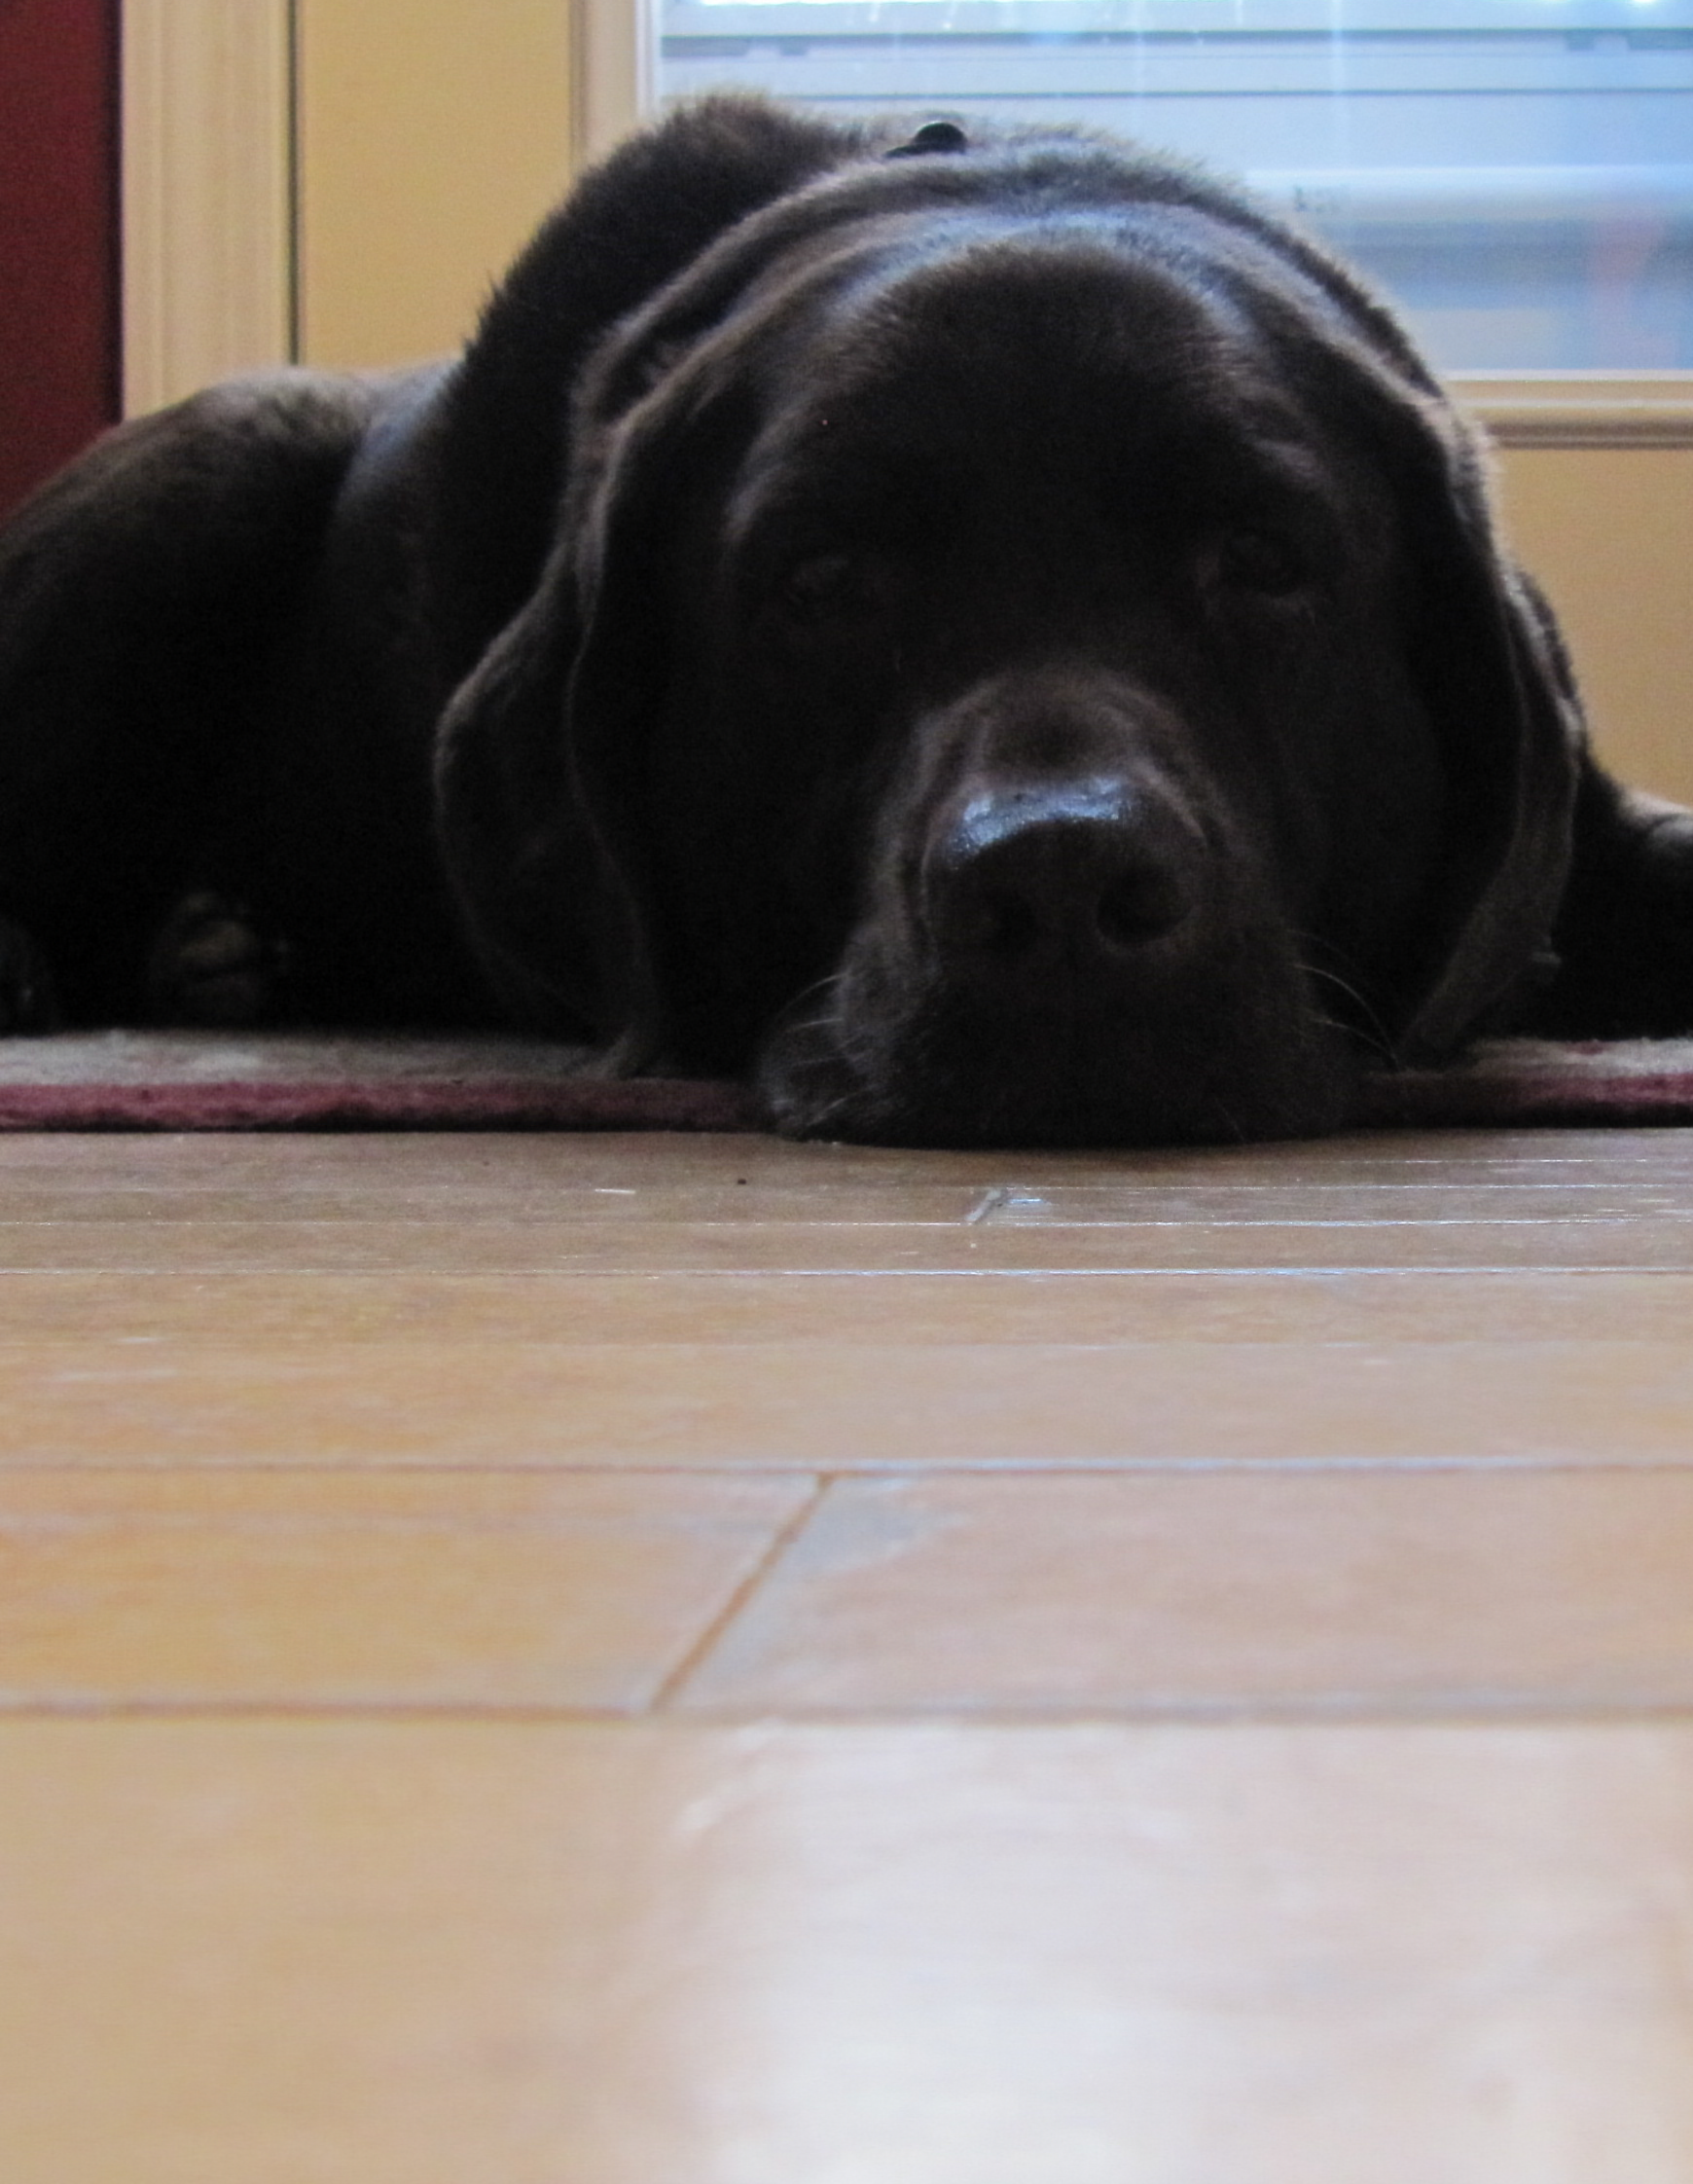
\includegraphics[width=.4\textwidth]{pix/suzy_cover_squeezed.png}}
\end{center}



\section{Source of plot\_action.sage}

The \inlinecode{plot_circle_action}
routine that we call above takes the four entries of the $\nbyn{2}$
matrix and returns a list of two graphics, showing the input and the
output.
Other parameters are the number of colors, and a flag giving whether
to plot a full circle or whether to plot just the top half circle (the 
default is to show the top half).

The driver routine determines the list of colors and 
calls a helper \inlinecode{color_circle_list}, 
given below, which returns a list of graphics.
Finally, the routine plots those graphics.
\lstinputlisting[firstline=38,lastline=49]{plot_action.sage}

The helper routine does the heavy lifting.
There are two global values to set graphic values.
The variable \inlinecode{CIRCLE_THICKNESS} sets the thickness of 
the plotted curve, in points (a printer's unit, here $1/72$~inch).
Similarly \inlinecode{DOT_SIZE} sets the size of the small empty circle.
This routine produces a parametrized curve $(x(t),y(t))$ and uses \Sage's
\inlinecode{parametric_plot} function to get the resulting graphic.
\lstinputlisting[firstline=4,lastline=35]{plot_action.sage}
If this routine is plotting the upper half circle then it adds the
small empty circle at the end to show that the image of $(-1,0)$
is not part of the graph.




\section{Source of img\_squeeze.sage}
We use the Python Image Library for reading and writing the graphic.
\lstinputlisting[firstline=2,lastline=2]{img_squeeze.sage}
The function
\inlinecode{img_squeeze}
takes three arguments:~the names of the two files, and
the cutoff real number between $0$ and~$1$ the gives the percentage 
of the singular values to retain in the sum.
\lstinputlisting[firstline=4,lastline=8]{img_squeeze.sage}

This function first brings the input data to a format where each
pixel is a triple 
$(\text{red}, \text{green},\text{blue})$ of integers that range from 
$0$ to~$255$.
It uses those numbers to build 
three Python arrays \inlinecode{rd}, \inlinecode{gr},
and \inlinecode{bl}, which then initialize the 
three \Sage{} matrices \inlinecode{RD},
\inlinecode{GR}, and~\inlinecode{BL}.
\lstinputlisting[firstline=9,lastline=25]{img_squeeze.sage}

The next step finds the Singular Value Decomposition of those three.
Out of curiosity, we have a look at the eight largest singular
values in the red matrix, the singular value where we make the cutoff,
and the eight smallest.
\lstinputlisting[firstline=26,lastline=38]{img_squeeze.sage}

Finally, for each matrix we compute the sum
$\sigma_1\cdot\vec{u}_1\trans{\vec{v}}_1+\sigma_2\cdot\vec{u}_2\trans{\vec{v}}_2
   +\cdots$
up through the cutoff index.
\lstinputlisting[firstline=39,lastline=58]{img_squeeze.sage}
% The code asks for the transpose of the
% \protect\inlinecode{U_RD.column(i)}, etc., which may seem to be a mistake.
% Remember that \protect\Sage{} favors rows for vectors, so this is how we
% make the $\vec{u}$ vector a column, while $\vec{v}$ is already a row.
% Because of this operation on the vector, the first time you run this
% code in a \protect\Sage{} session you may get a depreciation warning.

To finish, we put the data in the PNG format and save it to 
disk.
\lstinputlisting[firstline=59,lastline=67]{img_squeeze.sage}
This part of the routine takes a long time, in part because
the code is written to be easy to read rather than to be fast to run.

\endinput


TODO:
1) mention Sage matrices are not mutable in matrix introduction.
Is mutable discussed in Intro?

2) vectors have to be forced to be row or col

2) Need int() fcns?  copy() fcn?